\documentclass[1p]{elsarticle_modified}
%\bibliographystyle{elsarticle-num}

%\usepackage[colorlinks]{hyperref}
%\usepackage{abbrmath_seonhwa} %\Abb, \Ascr, \Acal ,\Abf, \Afrak
\usepackage{amsfonts}
\usepackage{amssymb}
\usepackage{amsmath}
\usepackage{amsthm}
\usepackage{scalefnt}
\usepackage{amsbsy}
\usepackage{kotex}
\usepackage{caption}
\usepackage{subfig}
\usepackage{color}
\usepackage{graphicx}
\usepackage{xcolor} %% white, black, red, green, blue, cyan, magenta, yellow
\usepackage{float}
\usepackage{setspace}
\usepackage{hyperref}

\usepackage{tikz}
\usetikzlibrary{arrows}

\usepackage{multirow}
\usepackage{array} % fixed length table
\usepackage{hhline}

%%%%%%%%%%%%%%%%%%%%%
\makeatletter
\renewcommand*\env@matrix[1][\arraystretch]{%
	\edef\arraystretch{#1}%
	\hskip -\arraycolsep
	\let\@ifnextchar\new@ifnextchar
	\array{*\c@MaxMatrixCols c}}
\makeatother %https://tex.stackexchange.com/questions/14071/how-can-i-increase-the-line-spacing-in-a-matrix
%%%%%%%%%%%%%%%

\usepackage[normalem]{ulem}

\newcommand{\msout}[1]{\ifmmode\text{\sout{\ensuremath{#1}}}\else\sout{#1}\fi}
%SOURCE: \msout is \stkout macro in https://tex.stackexchange.com/questions/20609/strikeout-in-math-mode

\newcommand{\cancel}[1]{
	\ifmmode
	{\color{red}\msout{#1}}
	\else
	{\color{red}\sout{#1}}
	\fi
}

\newcommand{\add}[1]{
	{\color{blue}\uwave{#1}}
}

\newcommand{\replace}[2]{
	\ifmmode
	{\color{red}\msout{#1}}{\color{blue}\uwave{#2}}
	\else
	{\color{red}\sout{#1}}{\color{blue}\uwave{#2}}
	\fi
}

\newcommand{\Sol}{\mathcal{S}} %segment
\newcommand{\D}{D} %diagram
\newcommand{\A}{\mathcal{A}} %arc


%%%%%%%%%%%%%%%%%%%%%%%%%%%%%5 test

\def\sl{\operatorname{\textup{SL}}(2,\Cbb)}
\def\psl{\operatorname{\textup{PSL}}(2,\Cbb)}
\def\quan{\mkern 1mu \triangleright \mkern 1mu}

\theoremstyle{definition}
\newtheorem{thm}{Theorem}[section]
\newtheorem{prop}[thm]{Proposition}
\newtheorem{lem}[thm]{Lemma}
\newtheorem{ques}[thm]{Question}
\newtheorem{cor}[thm]{Corollary}
\newtheorem{defn}[thm]{Definition}
\newtheorem{exam}[thm]{Example}
\newtheorem{rmk}[thm]{Remark}
\newtheorem{alg}[thm]{Algorithm}

\newcommand{\I}{\sqrt{-1}}
\begin{document}

%\begin{frontmatter}
%
%\title{Boundary parabolic representations of knots up to 8 crossings}
%
%%% Group authors per affiliation:
%\author{Yunhi Cho} 
%\address{Department of Mathematics, University of Seoul, Seoul, Korea}
%\ead{yhcho@uos.ac.kr}
%
%
%\author{Seonhwa Kim} %\fnref{s_kim}}
%\address{Center for Geometry and Physics, Institute for Basic Science, Pohang, 37673, Korea}
%\ead{ryeona17@ibs.re.kr}
%
%\author{Hyuk Kim}
%\address{Department of Mathematical Sciences, Seoul National University, Seoul 08826, Korea}
%\ead{hyukkim@snu.ac.kr}
%
%\author{Seokbeom Yoon}
%\address{Department of Mathematical Sciences, Seoul National University, Seoul, 08826,  Korea}
%\ead{sbyoon15@snu.ac.kr}
%
%\begin{abstract}
%We find all boundary parabolic representation of knots up to 8 crossings.
%
%\end{abstract}
%\begin{keyword}
%    \MSC[2010] 57M25 
%\end{keyword}
%
%\end{frontmatter}

%\linenumbers
%\tableofcontents
%
\newcommand\colored[1]{\textcolor{white}{\rule[-0.35ex]{0.8em}{1.4ex}}\kern-0.8em\color{red} #1}%
%\newcommand\colored[1]{\textcolor{white}{ #1}\kern-2.17ex	\textcolor{white}{ #1}\kern-1.81ex	\textcolor{white}{ #1}\kern-2.15ex\color{red}#1	}

{\Large $\underline{10_{64}~(K10a_{122})}$}

\setlength{\tabcolsep}{10pt}
\renewcommand{\arraystretch}{1.6}
\vspace{1cm}\begin{tabular}{m{100pt}>{\centering\arraybackslash}m{274pt}}
\multirow{5}{120pt}{
	\centering
	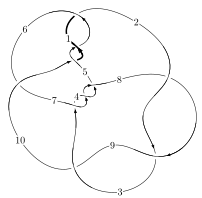
\includegraphics[width=112pt]{../../../GIT/diagram.site/Diagrams/png/148_10_64.png}\\
\ \ \ A knot diagram\footnotemark}&
\allowdisplaybreaks
\textbf{Linearized knot diagam} \\
\cline{2-2}
 &
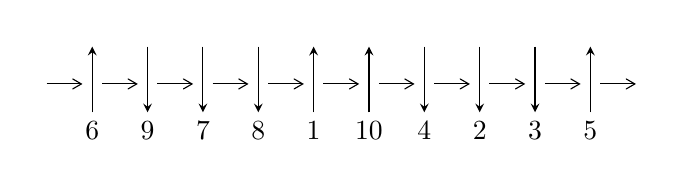
\begin{tikzpicture}[x=20pt, y=17pt]
	% nodes
	\node (C0) at (0, 0) {};
	\node (C1) at (1, 0) {};
	\node (C1U) at (1, +1) {};
	\node (C1D) at (1, -1) {6};

	\node (C2) at (2, 0) {};
	\node (C2U) at (2, +1) {};
	\node (C2D) at (2, -1) {9};

	\node (C3) at (3, 0) {};
	\node (C3U) at (3, +1) {};
	\node (C3D) at (3, -1) {7};

	\node (C4) at (4, 0) {};
	\node (C4U) at (4, +1) {};
	\node (C4D) at (4, -1) {8};

	\node (C5) at (5, 0) {};
	\node (C5U) at (5, +1) {};
	\node (C5D) at (5, -1) {1};

	\node (C6) at (6, 0) {};
	\node (C6U) at (6, +1) {};
	\node (C6D) at (6, -1) {10};

	\node (C7) at (7, 0) {};
	\node (C7U) at (7, +1) {};
	\node (C7D) at (7, -1) {4};

	\node (C8) at (8, 0) {};
	\node (C8U) at (8, +1) {};
	\node (C8D) at (8, -1) {2};

	\node (C9) at (9, 0) {};
	\node (C9U) at (9, +1) {};
	\node (C9D) at (9, -1) {3};

	\node (C10) at (10, 0) {};
	\node (C10U) at (10, +1) {};
	\node (C10D) at (10, -1) {5};
	\node (C11) at (11, 0) {};

	% arrows
	\draw[->,>={angle 60}]
	(C0) edge (C1) (C1) edge (C2) (C2) edge (C3) (C3) edge (C4) (C4) edge (C5) (C5) edge (C6) (C6) edge (C7) (C7) edge (C8) (C8) edge (C9) (C9) edge (C10) (C10) edge (C11) ;	\draw[->,>=stealth]
	(C1D) edge (C1U) (C2U) edge (C2D) (C3U) edge (C3D) (C4U) edge (C4D) (C5D) edge (C5U) (C6D) edge (C6U) (C7U) edge (C7D) (C8U) edge (C8D) (C9U) edge (C9D) (C10D) edge (C10U) ;
	\end{tikzpicture} \\
\hhline{~~} \\& 
\textbf{Solving Sequence} \\ \cline{2-2} 
 &
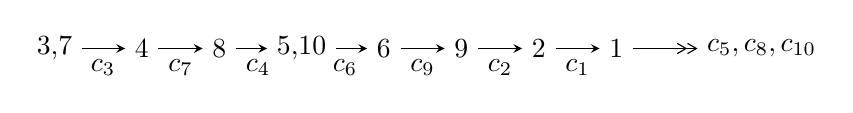
\begin{tikzpicture}[x=28pt, y=7pt]
	% node
	\node (A0) at (-1/8, 0) {3,7};
	\node (A1) at (1, 0) {4};
	\node (A2) at (2, 0) {8};
	\node (A3) at (49/16, 0) {5,10};
	\node (A4) at (33/8, 0) {6};
	\node (A5) at (41/8, 0) {9};
	\node (A6) at (49/8, 0) {2};
	\node (A7) at (57/8, 0) {1};
	\node (C1) at (1/2, -1) {$c_{3}$};
	\node (C2) at (3/2, -1) {$c_{7}$};
	\node (C3) at (5/2, -1) {$c_{4}$};
	\node (C4) at (29/8, -1) {$c_{6}$};
	\node (C5) at (37/8, -1) {$c_{9}$};
	\node (C6) at (45/8, -1) {$c_{2}$};
	\node (C7) at (53/8, -1) {$c_{1}$};
	\node (A8) at (9, 0) {$c_{5},c_{8},c_{10}$};

	% edge
	\draw[->,>=stealth]	
	(A0) edge (A1) (A1) edge (A2) (A2) edge (A3) (A3) edge (A4) (A4) edge (A5) (A5) edge (A6) (A6) edge (A7) ;
	\draw[->>,>={angle 60}]	
	(A7) edge (A8);
\end{tikzpicture} \\ 

\end{tabular} \\

\footnotetext{
The image of knot diagram is generated by the software ``\textbf{Draw programme}" developed by Andrew Bartholomew(\url{http://www.layer8.co.uk/maths/draw/index.htm\#Running-draw}), where we modified some parts for our purpose(\url{https://github.com/CATsTAILs/LinksPainter}).
}\phantom \\ \newline 
\centering \textbf{Ideals for irreducible components\footnotemark of $X_{\text{par}}$} 
 
\begin{align*}
I^u_{1}&=\langle 
b- u,\;- u^{10}- u^9+6 u^8+5 u^7-12 u^6-6 u^5+7 u^4-4 u^3+u^2+2 a+6 u+1,\\
\phantom{I^u_{1}}&\phantom{= \langle  }u^{12}+u^{11}-7 u^{10}-6 u^9+18 u^8+11 u^7-19 u^6-2 u^5+6 u^4-8 u^3+1\rangle \\
I^u_{2}&=\langle 
-79 u^{15}-74 u^{14}+\cdots+47 b-143,\;126 u^{15}+121 u^{14}+\cdots+47 a+425,\;u^{16}+u^{15}+\cdots+6 u-1\rangle \\
I^u_{3}&=\langle 
b+1,\;a,\;u-1\rangle \\
I^u_{4}&=\langle 
b-1,\;a^2-2,\;u+1\rangle \\
\\
\end{align*}
\raggedright * 4 irreducible components of $\dim_{\mathbb{C}}=0$, with total 31 representations.\\
\footnotetext{All coefficients of polynomials are rational numbers. But the coefficients are sometimes approximated in decimal forms when there is not enough margin.}
\newpage
\renewcommand{\arraystretch}{1}
\centering \section*{I. $I^u_{1}= \langle b- u,\;- u^{10}- u^9+\cdots+2 a+1,\;u^{12}+u^{11}+\cdots-8 u^3+1 \rangle$}
\flushleft \textbf{(i) Arc colorings}\\
\begin{tabular}{m{7pt} m{180pt} m{7pt} m{180pt} }
\flushright $a_{3}=$&$\begin{pmatrix}1\\0\end{pmatrix}$ \\
\flushright $a_{7}=$&$\begin{pmatrix}0\\u\end{pmatrix}$ \\
\flushright $a_{4}=$&$\begin{pmatrix}1\\u^2\end{pmatrix}$ \\
\flushright $a_{8}=$&$\begin{pmatrix}- u\\- u^3+u\end{pmatrix}$ \\
\flushright $a_{5}=$&$\begin{pmatrix}- u^2+1\\- u^4+2 u^2\end{pmatrix}$ \\
\flushright $a_{10}=$&$\begin{pmatrix}\frac{1}{2} u^{10}+\frac{1}{2} u^9+\cdots-3 u-\frac{1}{2}\\u\end{pmatrix}$ \\
\flushright $a_{6}=$&$\begin{pmatrix}\frac{1}{2} u^{11}-\frac{7}{2} u^9+\cdots-\frac{1}{2} u-\frac{1}{2}\\-\frac{1}{2} u^{10}-\frac{1}{2} u^9+\cdots+u+\frac{1}{2}\end{pmatrix}$ \\
\flushright $a_{9}=$&$\begin{pmatrix}\frac{1}{2} u^{10}+\frac{1}{2} u^9+\cdots-2 u-\frac{1}{2}\\u\end{pmatrix}$ \\
\flushright $a_{2}=$&$\begin{pmatrix}-\frac{1}{2} u^{11}-\frac{1}{2} u^{10}+\cdots+\frac{1}{2} u+1\\- u^2\end{pmatrix}$ \\
\flushright $a_{1}=$&$\begin{pmatrix}\frac{1}{2} u^{10}+\frac{1}{2} u^9+\cdots-2 u-\frac{1}{2}\\-\frac{1}{2} u^{10}+\frac{1}{2} u^9+\cdots+u+\frac{1}{2}\end{pmatrix}$\\&\end{tabular}
\flushleft \textbf{(ii) Obstruction class $= -1$}\\~\\
\flushleft \textbf{(iii) Cusp Shapes $= -2 u^{11}- u^{10}+15 u^9+4 u^8-41 u^7+2 u^6+46 u^5-25 u^4-14 u^3+23 u^2-4 u-1$}\\~\\
\newpage\renewcommand{\arraystretch}{1}
\flushleft \textbf{(iv) u-Polynomials at the component}\newline \\
\begin{tabular}{m{50pt}|m{274pt}}
Crossings & \hspace{64pt}u-Polynomials at each crossing \\
\hline $$\begin{aligned}c_{1},c_{5},c_{10}\end{aligned}$$&$\begin{aligned}
&u^{12}+3 u^{11}+\cdots+2 u-2
\end{aligned}$\\
\hline $$\begin{aligned}c_{2},c_{3},c_{4}\\c_{7},c_{8},c_{9}\end{aligned}$$&$\begin{aligned}
&u^{12}+u^{11}-7 u^{10}-6 u^9+18 u^8+11 u^7-19 u^6-2 u^5+6 u^4-8 u^3+1
\end{aligned}$\\
\hline $$\begin{aligned}c_{6}\end{aligned}$$&$\begin{aligned}
&u^{12}-9 u^{11}+\cdots+102 u-22
\end{aligned}$\\
\hline
\end{tabular}\\~\\
\newpage\renewcommand{\arraystretch}{1}
\flushleft \textbf{(v) Riley Polynomials at the component}\newline \\
\begin{tabular}{m{50pt}|m{274pt}}
Crossings & \hspace{64pt}Riley Polynomials at each crossing \\
\hline $$\begin{aligned}c_{1},c_{5},c_{10}\end{aligned}$$&$\begin{aligned}
&y^{12}-11 y^{11}+\cdots+20 y+4
\end{aligned}$\\
\hline $$\begin{aligned}c_{2},c_{3},c_{4}\\c_{7},c_{8},c_{9}\end{aligned}$$&$\begin{aligned}
&y^{12}-15 y^{11}+\cdots+12 y^2+1
\end{aligned}$\\
\hline $$\begin{aligned}c_{6}\end{aligned}$$&$\begin{aligned}
&y^{12}+y^{11}+\cdots+1300 y+484
\end{aligned}$\\
\hline
\end{tabular}\\~\\
\newpage\flushleft \textbf{(vi) Complex Volumes and Cusp Shapes}
$$\begin{array}{c|c|c}  
\text{Solutions to }I^u_{1}& \I (\text{vol} + \sqrt{-1}CS) & \text{Cusp shape}\\
 \hline 
\begin{aligned}
u &= \phantom{-}0.298602 + 0.646764 I \\
a &= -0.45214 - 1.66459 I \\
b &= \phantom{-}0.298602 + 0.646764 I\end{aligned}
 & \phantom{-}4.65271 - 3.28049 I & \phantom{-}2.99435 + 5.25300 I \\ \hline\begin{aligned}
u &= \phantom{-}0.298602 - 0.646764 I \\
a &= -0.45214 + 1.66459 I \\
b &= \phantom{-}0.298602 - 0.646764 I\end{aligned}
 & \phantom{-}4.65271 + 3.28049 I & \phantom{-}2.99435 - 5.25300 I \\ \hline\begin{aligned}
u &= \phantom{-}1.37505\phantom{ +0.000000I} \\
a &= \phantom{-}1.71226\phantom{ +0.000000I} \\
b &= \phantom{-}1.37505\phantom{ +0.000000I}\end{aligned}
 & -1.04846\phantom{ +0.000000I} & -6.10990\phantom{ +0.000000I} \\ \hline\begin{aligned}
u &= \phantom{-}0.527999\phantom{ +0.000000I} \\
a &= -1.99219\phantom{ +0.000000I} \\
b &= \phantom{-}0.527999\phantom{ +0.000000I}\end{aligned}
 & \phantom{-}3.24831\phantom{ +0.000000I} & \phantom{-}0.826740\phantom{ +0.000000I} \\ \hline\begin{aligned}
u &= -1.50349 + 0.33368 I \\
a &= -0.268985 - 1.300570 I \\
b &= -1.50349 + 0.33368 I\end{aligned}
 & -7.04968 + 10.86810 I & -5.35737 - 5.74032 I \\ \hline\begin{aligned}
u &= -1.50349 - 0.33368 I \\
a &= -0.268985 + 1.300570 I \\
b &= -1.50349 - 0.33368 I\end{aligned}
 & -7.04968 - 10.86810 I & -5.35737 + 5.74032 I \\ \hline\begin{aligned}
u &= -1.54202 + 0.13644 I \\
a &= -0.585241 - 0.594215 I \\
b &= -1.54202 + 0.13644 I\end{aligned}
 & -10.10900 + 1.20346 I & -7.47592 + 0.43067 I \\ \hline\begin{aligned}
u &= -1.54202 - 0.13644 I \\
a &= -0.585241 + 0.594215 I \\
b &= -1.54202 - 0.13644 I\end{aligned}
 & -10.10900 - 1.20346 I & -7.47592 - 0.43067 I \\ \hline\begin{aligned}
u &= -0.245576 + 0.368193 I \\
a &= \phantom{-}0.577777 - 1.108910 I \\
b &= -0.245576 + 0.368193 I\end{aligned}
 & -0.111574 + 0.933771 I & -2.28396 - 7.38290 I \\ \hline\begin{aligned}
u &= -0.245576 - 0.368193 I \\
a &= \phantom{-}0.577777 + 1.108910 I \\
b &= -0.245576 - 0.368193 I\end{aligned}
 & -0.111574 - 0.933771 I & -2.28396 + 7.38290 I\\
 \hline 
 \end{array}$$\newpage$$\begin{array}{c|c|c}  
\text{Solutions to }I^u_{1}& \I (\text{vol} + \sqrt{-1}CS) & \text{Cusp shape}\\
 \hline 
\begin{aligned}
u &= \phantom{-}1.54096 + 0.25161 I \\
a &= \phantom{-}0.368549 - 0.997077 I \\
b &= \phantom{-}1.54096 + 0.25161 I\end{aligned}
 & -12.33390 - 6.28413 I & -9.23554 + 3.97965 I \\ \hline\begin{aligned}
u &= \phantom{-}1.54096 - 0.25161 I \\
a &= \phantom{-}0.368549 + 0.997077 I \\
b &= \phantom{-}1.54096 - 0.25161 I\end{aligned}
 & -12.33390 + 6.28413 I & -9.23554 - 3.97965 I\\
 \hline 
 \end{array}$$\newpage\newpage\renewcommand{\arraystretch}{1}
\centering \section*{II. $I^u_{2}= \langle -79 u^{15}-74 u^{14}+\cdots+47 b-143,\;126 u^{15}+121 u^{14}+\cdots+47 a+425,\;u^{16}+u^{15}+\cdots+6 u-1 \rangle$}
\flushleft \textbf{(i) Arc colorings}\\
\begin{tabular}{m{7pt} m{180pt} m{7pt} m{180pt} }
\flushright $a_{3}=$&$\begin{pmatrix}1\\0\end{pmatrix}$ \\
\flushright $a_{7}=$&$\begin{pmatrix}0\\u\end{pmatrix}$ \\
\flushright $a_{4}=$&$\begin{pmatrix}1\\u^2\end{pmatrix}$ \\
\flushright $a_{8}=$&$\begin{pmatrix}- u\\- u^3+u\end{pmatrix}$ \\
\flushright $a_{5}=$&$\begin{pmatrix}- u^2+1\\- u^4+2 u^2\end{pmatrix}$ \\
\flushright $a_{10}=$&$\begin{pmatrix}-2.68085 u^{15}-2.57447 u^{14}+\cdots+14.1277 u-9.04255\\1.68085 u^{15}+1.57447 u^{14}+\cdots-8.12766 u+3.04255\end{pmatrix}$ \\
\flushright $a_{6}=$&$\begin{pmatrix}-3.06383 u^{15}-4.08511 u^{14}+\cdots+23.5745 u-12.1915\\0.382979 u^{15}+1.51064 u^{14}+\cdots-8.44681 u+3.14894\end{pmatrix}$ \\
\flushright $a_{9}=$&$\begin{pmatrix}- u^{15}- u^{14}+\cdots+6 u-6\\1.68085 u^{15}+1.57447 u^{14}+\cdots-8.12766 u+3.04255\end{pmatrix}$ \\
\flushright $a_{2}=$&$\begin{pmatrix}3.04255 u^{15}+4.72340 u^{14}+\cdots-26.3830 u+11.1277\\-0.106383 u^{15}+1.19149 u^{14}+\cdots-7.04255 u+0.680851\end{pmatrix}$ \\
\flushright $a_{1}=$&$\begin{pmatrix}-1.14894 u^{15}-1.53191 u^{14}+\cdots+10.3404 u-6.44681\\2.04255 u^{15}+2.72340 u^{14}+\cdots-12.3830 u+4.12766\end{pmatrix}$\\&\end{tabular}
\flushleft \textbf{(ii) Obstruction class $= -1$}\\~\\
\flushleft \textbf{(iii) Cusp Shapes $= -\frac{4}{47} u^{15}+\frac{120}{47} u^{14}+\frac{64}{47} u^{13}-\frac{652}{47} u^{12}+\frac{36}{47} u^{11}+28 u^{10}-\frac{856}{47} u^9-\frac{1120}{47} u^8+\frac{1372}{47} u^7+\frac{364}{47} u^6-\frac{708}{47} u^5-\frac{456}{47} u^4+\frac{928}{47} u^3+\frac{412}{47} u^2-\frac{904}{47} u+\frac{270}{47}$}\\~\\
\newpage\renewcommand{\arraystretch}{1}
\flushleft \textbf{(iv) u-Polynomials at the component}\newline \\
\begin{tabular}{m{50pt}|m{274pt}}
Crossings & \hspace{64pt}u-Polynomials at each crossing \\
\hline $$\begin{aligned}c_{1},c_{5},c_{10}\end{aligned}$$&$\begin{aligned}
&(u^8- u^7-3 u^6+2 u^5+3 u^4-2 u-1)^2
\end{aligned}$\\
\hline $$\begin{aligned}c_{2},c_{3},c_{4}\\c_{7},c_{8},c_{9}\end{aligned}$$&$\begin{aligned}
&u^{16}+u^{15}+\cdots+6 u-1
\end{aligned}$\\
\hline $$\begin{aligned}c_{6}\end{aligned}$$&$\begin{aligned}
&(u^8+3 u^7+7 u^6+10 u^5+11 u^4+10 u^3+6 u^2+4 u+1)^2
\end{aligned}$\\
\hline
\end{tabular}\\~\\
\newpage\renewcommand{\arraystretch}{1}
\flushleft \textbf{(v) Riley Polynomials at the component}\newline \\
\begin{tabular}{m{50pt}|m{274pt}}
Crossings & \hspace{64pt}Riley Polynomials at each crossing \\
\hline $$\begin{aligned}c_{1},c_{5},c_{10}\end{aligned}$$&$\begin{aligned}
&(y^8-7 y^7+19 y^6-22 y^5+3 y^4+14 y^3-6 y^2-4 y+1)^2
\end{aligned}$\\
\hline $$\begin{aligned}c_{2},c_{3},c_{4}\\c_{7},c_{8},c_{9}\end{aligned}$$&$\begin{aligned}
&y^{16}-13 y^{15}+\cdots-24 y+1
\end{aligned}$\\
\hline $$\begin{aligned}c_{6}\end{aligned}$$&$\begin{aligned}
&(y^8+5 y^7+11 y^6+6 y^5-17 y^4-34 y^3-22 y^2-4 y+1)^2
\end{aligned}$\\
\hline
\end{tabular}\\~\\
\newpage\flushleft \textbf{(vi) Complex Volumes and Cusp Shapes}
$$\begin{array}{c|c|c}  
\text{Solutions to }I^u_{2}& \I (\text{vol} + \sqrt{-1}CS) & \text{Cusp shape}\\
 \hline 
\begin{aligned}
u &= \phantom{-}0.396638 + 0.883588 I \\
a &= \phantom{-}1.00561 + 1.17006 I \\
b &= -1.42845 - 0.22812 I\end{aligned}
 & -0.91019 - 6.44354 I & -2.57155 + 5.29417 I \\ \hline\begin{aligned}
u &= \phantom{-}0.396638 - 0.883588 I \\
a &= \phantom{-}1.00561 - 1.17006 I \\
b &= -1.42845 + 0.22812 I\end{aligned}
 & -0.91019 + 6.44354 I & -2.57155 - 5.29417 I \\ \hline\begin{aligned}
u &= \phantom{-}0.825972 + 0.646815 I \\
a &= \phantom{-}0.646365 + 0.503837 I \\
b &= -1.396840 + 0.083857 I\end{aligned}
 & -2.24921 + 1.13123 I & -4.58478 - 0.51079 I \\ \hline\begin{aligned}
u &= \phantom{-}0.825972 - 0.646815 I \\
a &= \phantom{-}0.646365 - 0.503837 I \\
b &= -1.396840 - 0.083857 I\end{aligned}
 & -2.24921 - 1.13123 I & -4.58478 + 0.51079 I \\ \hline\begin{aligned}
u &= -0.558144 + 0.766237 I \\
a &= -0.792286 + 0.953005 I \\
b &= \phantom{-}1.41338 - 0.10034 I\end{aligned}
 & -5.44928 + 2.57849 I & -7.72292 - 3.56796 I \\ \hline\begin{aligned}
u &= -0.558144 - 0.766237 I \\
a &= -0.792286 - 0.953005 I \\
b &= \phantom{-}1.41338 + 0.10034 I\end{aligned}
 & -5.44928 - 2.57849 I & -7.72292 + 3.56796 I \\ \hline\begin{aligned}
u &= \phantom{-}0.858124\phantom{ +0.000000I} \\
a &= -1.40539\phantom{ +0.000000I} \\
b &= \phantom{-}0.240055\phantom{ +0.000000I}\end{aligned}
 & \phantom{-}3.21286\phantom{ +0.000000I} & \phantom{-}1.86400\phantom{ +0.000000I} \\ \hline\begin{aligned}
u &= -1.15431\phantom{ +0.000000I} \\
a &= \phantom{-}0.315320\phantom{ +0.000000I} \\
b &= \phantom{-}0.551002\phantom{ +0.000000I}\end{aligned}
 & -2.44483\phantom{ +0.000000I} & -0.105540\phantom{ +0.000000I} \\ \hline\begin{aligned}
u &= -1.396840 + 0.083857 I \\
a &= -0.112641 - 0.603991 I \\
b &= \phantom{-}0.825972 + 0.646815 I\end{aligned}
 & -2.24921 + 1.13123 I & -4.58478 - 0.51079 I \\ \hline\begin{aligned}
u &= -1.396840 - 0.083857 I \\
a &= -0.112641 + 0.603991 I \\
b &= \phantom{-}0.825972 - 0.646815 I\end{aligned}
 & -2.24921 - 1.13123 I & -4.58478 + 0.51079 I\\
 \hline 
 \end{array}$$\newpage$$\begin{array}{c|c|c}  
\text{Solutions to }I^u_{2}& \I (\text{vol} + \sqrt{-1}CS) & \text{Cusp shape}\\
 \hline 
\begin{aligned}
u &= \phantom{-}1.41338 + 0.10034 I \\
a &= -0.145831 + 0.816217 I \\
b &= -0.558144 - 0.766237 I\end{aligned}
 & -5.44928 - 2.57849 I & -7.72292 + 3.56796 I \\ \hline\begin{aligned}
u &= \phantom{-}1.41338 - 0.10034 I \\
a &= -0.145831 - 0.816217 I \\
b &= -0.558144 + 0.766237 I\end{aligned}
 & -5.44928 + 2.57849 I & -7.72292 - 3.56796 I \\ \hline\begin{aligned}
u &= -1.42845 + 0.22812 I \\
a &= \phantom{-}0.286014 + 0.992605 I \\
b &= \phantom{-}0.396638 - 0.883588 I\end{aligned}
 & -0.91019 + 6.44354 I & -2.57155 - 5.29417 I \\ \hline\begin{aligned}
u &= -1.42845 - 0.22812 I \\
a &= \phantom{-}0.286014 - 0.992605 I \\
b &= \phantom{-}0.396638 + 0.883588 I\end{aligned}
 & -0.91019 - 6.44354 I & -2.57155 + 5.29417 I \\ \hline\begin{aligned}
u &= \phantom{-}0.551002\phantom{ +0.000000I} \\
a &= -0.660569\phantom{ +0.000000I} \\
b &= -1.15431\phantom{ +0.000000I}\end{aligned}
 & -2.44483\phantom{ +0.000000I} & -0.105540\phantom{ +0.000000I} \\ \hline\begin{aligned}
u &= \phantom{-}0.240055\phantom{ +0.000000I} \\
a &= -5.02383\phantom{ +0.000000I} \\
b &= \phantom{-}0.858124\phantom{ +0.000000I}\end{aligned}
 & \phantom{-}3.21286\phantom{ +0.000000I} & \phantom{-}1.86400\phantom{ +0.000000I}\\
 \hline 
 \end{array}$$\newpage\newpage\renewcommand{\arraystretch}{1}
\centering \section*{III. $I^u_{3}= \langle b+1,\;a,\;u-1 \rangle$}
\flushleft \textbf{(i) Arc colorings}\\
\begin{tabular}{m{7pt} m{180pt} m{7pt} m{180pt} }
\flushright $a_{3}=$&$\begin{pmatrix}1\\0\end{pmatrix}$ \\
\flushright $a_{7}=$&$\begin{pmatrix}0\\1\end{pmatrix}$ \\
\flushright $a_{4}=$&$\begin{pmatrix}1\\1\end{pmatrix}$ \\
\flushright $a_{8}=$&$\begin{pmatrix}-1\\0\end{pmatrix}$ \\
\flushright $a_{5}=$&$\begin{pmatrix}0\\1\end{pmatrix}$ \\
\flushright $a_{10}=$&$\begin{pmatrix}0\\-1\end{pmatrix}$ \\
\flushright $a_{6}=$&$\begin{pmatrix}0\\1\end{pmatrix}$ \\
\flushright $a_{9}=$&$\begin{pmatrix}-1\\-1\end{pmatrix}$ \\
\flushright $a_{2}=$&$\begin{pmatrix}0\\-1\end{pmatrix}$ \\
\flushright $a_{1}=$&$\begin{pmatrix}0\\-1\end{pmatrix}$\\&\end{tabular}
\flushleft \textbf{(ii) Obstruction class $= 1$}\\~\\
\flushleft \textbf{(iii) Cusp Shapes $= -12$}\\~\\
\newpage\renewcommand{\arraystretch}{1}
\flushleft \textbf{(iv) u-Polynomials at the component}\newline \\
\begin{tabular}{m{50pt}|m{274pt}}
Crossings & \hspace{64pt}u-Polynomials at each crossing \\
\hline $$\begin{aligned}c_{1},c_{5},c_{6}\\c_{10}\end{aligned}$$&$\begin{aligned}
&u
\end{aligned}$\\
\hline $$\begin{aligned}c_{2},c_{7}\end{aligned}$$&$\begin{aligned}
&u+1
\end{aligned}$\\
\hline $$\begin{aligned}c_{3},c_{4},c_{8}\\c_{9}\end{aligned}$$&$\begin{aligned}
&u-1
\end{aligned}$\\
\hline
\end{tabular}\\~\\
\newpage\renewcommand{\arraystretch}{1}
\flushleft \textbf{(v) Riley Polynomials at the component}\newline \\
\begin{tabular}{m{50pt}|m{274pt}}
Crossings & \hspace{64pt}Riley Polynomials at each crossing \\
\hline $$\begin{aligned}c_{1},c_{5},c_{6}\\c_{10}\end{aligned}$$&$\begin{aligned}
&y
\end{aligned}$\\
\hline $$\begin{aligned}c_{2},c_{3},c_{4}\\c_{7},c_{8},c_{9}\end{aligned}$$&$\begin{aligned}
&y-1
\end{aligned}$\\
\hline
\end{tabular}\\~\\
\newpage\flushleft \textbf{(vi) Complex Volumes and Cusp Shapes}
$$\begin{array}{c|c|c}  
\text{Solutions to }I^u_{3}& \I (\text{vol} + \sqrt{-1}CS) & \text{Cusp shape}\\
 \hline 
\begin{aligned}
u &= \phantom{-}1.00000\phantom{ +0.000000I} \\
a &= \phantom{-0.000000 } 0 \\
b &= -1.00000\phantom{ +0.000000I}\end{aligned}
 & -3.28987\phantom{ +0.000000I} & -12.0000\phantom{ +0.000000I}\\
 \hline 
 \end{array}$$\newpage\newpage\renewcommand{\arraystretch}{1}
\centering \section*{IV. $I^u_{4}= \langle b-1,\;a^2-2,\;u+1 \rangle$}
\flushleft \textbf{(i) Arc colorings}\\
\begin{tabular}{m{7pt} m{180pt} m{7pt} m{180pt} }
\flushright $a_{3}=$&$\begin{pmatrix}1\\0\end{pmatrix}$ \\
\flushright $a_{7}=$&$\begin{pmatrix}0\\-1\end{pmatrix}$ \\
\flushright $a_{4}=$&$\begin{pmatrix}1\\1\end{pmatrix}$ \\
\flushright $a_{8}=$&$\begin{pmatrix}1\\0\end{pmatrix}$ \\
\flushright $a_{5}=$&$\begin{pmatrix}0\\1\end{pmatrix}$ \\
\flushright $a_{10}=$&$\begin{pmatrix}a\\1\end{pmatrix}$ \\
\flushright $a_{6}=$&$\begin{pmatrix}2\\a-1\end{pmatrix}$ \\
\flushright $a_{9}=$&$\begin{pmatrix}a+1\\1\end{pmatrix}$ \\
\flushright $a_{2}=$&$\begin{pmatrix}- a\\-1\end{pmatrix}$ \\
\flushright $a_{1}=$&$\begin{pmatrix}a\\- a+1\end{pmatrix}$\\&\end{tabular}
\flushleft \textbf{(ii) Obstruction class $= 1$}\\~\\
\flushleft \textbf{(iii) Cusp Shapes $= -4$}\\~\\
\newpage\renewcommand{\arraystretch}{1}
\flushleft \textbf{(iv) u-Polynomials at the component}\newline \\
\begin{tabular}{m{50pt}|m{274pt}}
Crossings & \hspace{64pt}u-Polynomials at each crossing \\
\hline $$\begin{aligned}c_{1},c_{5},c_{6}\\c_{10}\end{aligned}$$&$\begin{aligned}
&u^2-2
\end{aligned}$\\
\hline $$\begin{aligned}c_{2},c_{7}\end{aligned}$$&$\begin{aligned}
&(u-1)^2
\end{aligned}$\\
\hline $$\begin{aligned}c_{3},c_{4},c_{8}\\c_{9}\end{aligned}$$&$\begin{aligned}
&(u+1)^2
\end{aligned}$\\
\hline
\end{tabular}\\~\\
\newpage\renewcommand{\arraystretch}{1}
\flushleft \textbf{(v) Riley Polynomials at the component}\newline \\
\begin{tabular}{m{50pt}|m{274pt}}
Crossings & \hspace{64pt}Riley Polynomials at each crossing \\
\hline $$\begin{aligned}c_{1},c_{5},c_{6}\\c_{10}\end{aligned}$$&$\begin{aligned}
&(y-2)^2
\end{aligned}$\\
\hline $$\begin{aligned}c_{2},c_{3},c_{4}\\c_{7},c_{8},c_{9}\end{aligned}$$&$\begin{aligned}
&(y-1)^2
\end{aligned}$\\
\hline
\end{tabular}\\~\\
\newpage\flushleft \textbf{(vi) Complex Volumes and Cusp Shapes}
$$\begin{array}{c|c|c}  
\text{Solutions to }I^u_{4}& \I (\text{vol} + \sqrt{-1}CS) & \text{Cusp shape}\\
 \hline 
\begin{aligned}
u &= -1.00000\phantom{ +0.000000I} \\
a &= \phantom{-}1.41421\phantom{ +0.000000I} \\
b &= \phantom{-}1.00000\phantom{ +0.000000I}\end{aligned}
 & \phantom{-}1.64493\phantom{ +0.000000I} & -4.00000\phantom{ +0.000000I} \\ \hline\begin{aligned}
u &= -1.00000\phantom{ +0.000000I} \\
a &= -1.41421\phantom{ +0.000000I} \\
b &= \phantom{-}1.00000\phantom{ +0.000000I}\end{aligned}
 & \phantom{-}1.64493\phantom{ +0.000000I} & -4.00000\phantom{ +0.000000I}\\
 \hline 
 \end{array}$$\newpage
\newpage\renewcommand{\arraystretch}{1}
\centering \section*{ V. u-Polynomials}
\begin{tabular}{m{50pt}|m{274pt}}
Crossings & \hspace{64pt}u-Polynomials at each crossing \\
\hline $$\begin{aligned}c_{1},c_{5},c_{10}\end{aligned}$$&$\begin{aligned}
&u(u^2-2)(u^8- u^7-3 u^6+2 u^5+3 u^4-2 u-1)^2\\
&\cdot(u^{12}+3 u^{11}+\cdots+2 u-2)
\end{aligned}$\\
\hline $$\begin{aligned}c_{2},c_{7}\end{aligned}$$&$\begin{aligned}
&(u-1)^2(u+1)\\
&\cdot(u^{12}+u^{11}-7 u^{10}-6 u^9+18 u^8+11 u^7-19 u^6-2 u^5+6 u^4-8 u^3+1)\\
&\cdot(u^{16}+u^{15}+\cdots+6 u-1)
\end{aligned}$\\
\hline $$\begin{aligned}c_{3},c_{4},c_{8}\\c_{9}\end{aligned}$$&$\begin{aligned}
&(u-1)(u+1)^2\\
&\cdot(u^{12}+u^{11}-7 u^{10}-6 u^9+18 u^8+11 u^7-19 u^6-2 u^5+6 u^4-8 u^3+1)\\
&\cdot(u^{16}+u^{15}+\cdots+6 u-1)
\end{aligned}$\\
\hline $$\begin{aligned}c_{6}\end{aligned}$$&$\begin{aligned}
&u(u^2-2)(u^8+3 u^7+7 u^6+10 u^5+11 u^4+10 u^3+6 u^2+4 u+1)^2\\
&\cdot(u^{12}-9 u^{11}+\cdots+102 u-22)
\end{aligned}$\\
\hline
\end{tabular}\newpage\renewcommand{\arraystretch}{1}
\centering \section*{ VI. Riley Polynomials}
\begin{tabular}{m{50pt}|m{274pt}}
Crossings & \hspace{64pt}Riley Polynomials at each crossing \\
\hline $$\begin{aligned}c_{1},c_{5},c_{10}\end{aligned}$$&$\begin{aligned}
&y(y-2)^2(y^8-7 y^7+19 y^6-22 y^5+3 y^4+14 y^3-6 y^2-4 y+1)^2\\
&\cdot(y^{12}-11 y^{11}+\cdots+20 y+4)
\end{aligned}$\\
\hline $$\begin{aligned}c_{2},c_{3},c_{4}\\c_{7},c_{8},c_{9}\end{aligned}$$&$\begin{aligned}
&((y-1)^3)(y^{12}-15 y^{11}+\cdots+12 y^2+1)(y^{16}-13 y^{15}+\cdots-24 y+1)
\end{aligned}$\\
\hline $$\begin{aligned}c_{6}\end{aligned}$$&$\begin{aligned}
&y(y-2)^2(y^8+5 y^7+11 y^6+6 y^5-17 y^4-34 y^3-22 y^2-4 y+1)^2\\
&\cdot(y^{12}+y^{11}+\cdots+1300 y+484)
\end{aligned}$\\
\hline
\end{tabular}
\vskip 2pc
\end{document}